\documentclass[12pt]{article}
\usepackage[utf8]{inputenc}
\usepackage{listings}
\usepackage{xcolor}
\usepackage{float}

\lstdefinestyle{mystyle}{
    belowcaptionskip=1\baselineskip,
    breaklines=true,
    frame=L,
    numbers=left,
    numbersep=10pt,
    xleftmargin=\parindent,
    showstringspaces=false,
    basicstyle=\footnotesize\ttfamily,
    keywordstyle=\bfseries\color{purple},
    commentstyle=\itshape\color{green},
    identifierstyle=\color{blue},
    stringstyle=\color{orange},
}

\lstset{style=mystyle}

\title{Analysis and Design of Algorithms}
\author{Carlos Esteban Guerrero Robles}
\date{06 April 2019}

\usepackage{natbib}
\usepackage{graphicx}
\usepackage{hyperref}
\usepackage{graphicx}
\graphicspath{ {src/} }

\begin{document}

\maketitle

\section{Warm up}

Lets modify the classic merge sort algorithm a little bit. What happens if instead of splitting the array in 2 parts we divide it in 3? You can assume that exists a three-way merge subroutine. What is the overall asymptotic running time of this algorithm?

\textbf{Answer:}

If we divide the array in 3 parts it will result in the reduction of the height of the division tree. But the steps of the three-way merge subroutine will be the same as the two-way merge subroutine, because they need necessarily to pass through all the array; however, the number of comparison in the subroutine will me more (at most three).\\

Based on that the running time will be:\\
$c*sizeArray(heightDivisionTree)+c*sizearray$\\
$c*n(log_3n)+c*n$\\

So the overall asymptotic running time will be:\\
$\Theta(nlog_3n)$\\

Even if looks like the three way method is more efficient than the normal merge sort, the actual time will be higher because the number of comparison in the sub-routine is more as mentioned before.

\emph{BONUS:} Implement the three-way merge sort algorithm.\\

\textbf{Answer:}

\emph{Three-way Merge Sub-routine:}
\lstinputlisting[language=c++]{src/p1/tWayM.h}

\emph{Three-way Merge Sort:}
\lstinputlisting[language=c++]{src/p1/tWayMS.h}

\emph{Main test:}
\lstinputlisting[language=c++]{src/p1/p1.cpp}

\section{Competitive programming}

Welcome to your first competitive programming problem!!!

\begin{itemize}
    \item Sign-up in Uva Online Judge (\url{https://uva.onlinejudge.org}) and in CodeChef if you want (we will use it later).
    \item Rest easy! This is not a contest, it is just an introductory problem. Your first problem is located in the ``Problems Section'' and is \textbf{100 - The 3n + 1 problem}.\\

    \textbf{Answer: }\\
    \lstinputlisting[language=c++]{src/p2/p2_100.cpp}

    \begin{figure}[H]
        \centering
        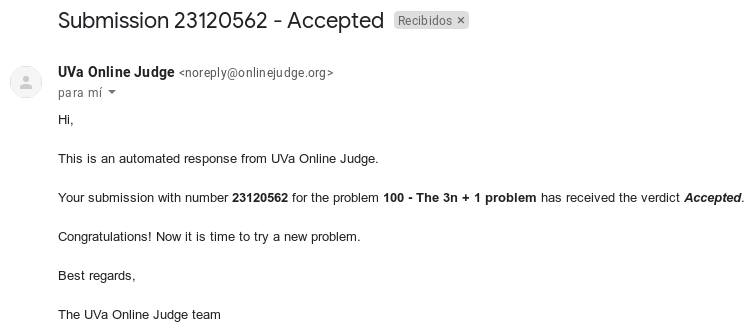
\includegraphics[scale=0.5]{p2/ss/p2_100.png}
        \caption{Problem 100 accepted by Uva}
        \label{p2_100}
    \end{figure}

    \item Once that you finish with that problem continue with \textbf{458 - The Decoder}. Again, this problem is just to build your confidence in competitive programming.

    \textbf{Answer: }\\
    \lstinputlisting[language=c++]{src/p2/p2_458.cpp}
    \begin{figure}[H]
        \centering
        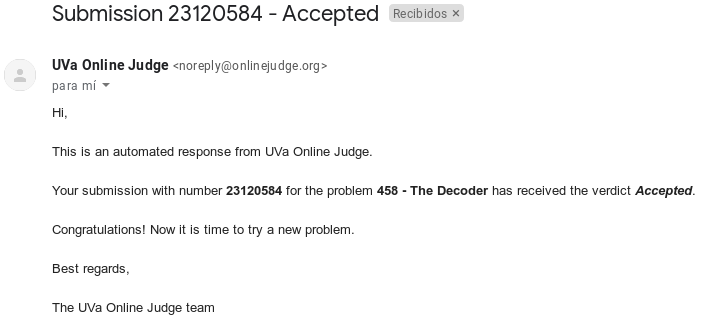
\includegraphics[scale=0.5]{p2/ss/p2_458.png}
        \caption{Problem 458 accepted by Uva}
        \label{p2_458}
    \end{figure}

    \item \emph{BONUS:} \textbf{10855 - Rotated squares}

    \textbf{Answer: }\\
    \lstinputlisting[language=c++]{src/p2/p2_10855.cpp}
    \begin{figure}[H]
        \centering
        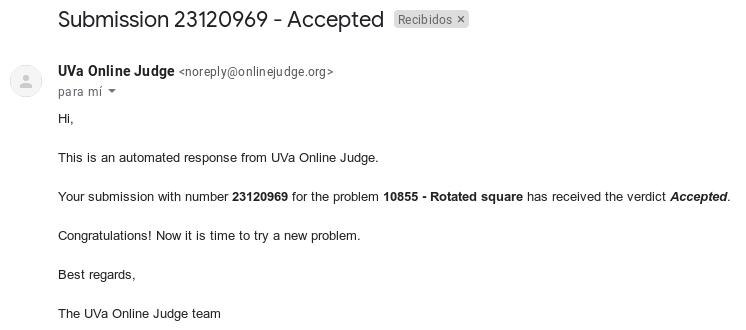
\includegraphics[scale=0.5]{p2/ss/p2_10855.png}
        \caption{Problem 10855 accepted by Uva}
        \label{p2_10855}
    \end{figure}

\end{itemize}

\section{Simulation}

Write a program to find the minimum input size for which the merge sort algorithm always beats the insertion sort.

\begin{itemize}
    \item Implement the insertion sort algorithm

    \textbf{Answer: }\\
    \lstinputlisting[language=c++]{src/p3/iSort.h}

    \item Implement the merge sort algorithm

    \textbf{Answer: }\\
    \lstinputlisting[language=c++]{src/p3/mSort.h}

    \item Just compare them? No !!! Run some simulations or tests and find the average input size for which the merge sort is an asymptotically ``better'' sorting algorithm.

    \textbf{Answer: }\\
    \lstinputlisting[language=c++]{src/p3/p3_1.cpp}

    \emph{Comments: }\\
    In order to have a well designed experiment I implement a random vector generator ramdomIG() (the vector is the same for both algorithms), a function to obtain a mean execution time of both algorithms testPS() (the size of the sample was 100). Also in the main function, there is a two loops; the first one is to find the firs input size for which the merge sort is asymptotically better, and in order to be sure that for higher input size merge sort continues being better than insertion exist the second loop. That loop demand that for an input size $n$ where merge sort is better than insertion sort, all the $n/2$ higher values of input size need to maintain the condition, if it does not accomplish continues searching a correct $n$ value.\\
    Also to have the chance of plot the experiment, all the input sizes and mean times of both algorithms are saved in a "test\_1.txt" file. There is its content:

    \lstinputlisting{src/p3/tests_1.txt}

\end{itemize}

Note: Include (.tex) and attach(.cpp) your source code and use a dockerfile to interact with python and plot your results.\\

\emph{BONUS:} Compare both algorithms against any other sorting algorithm

\textbf{Answer: }\\
I chose the selection sort as other algorithm to be compare against the insertion and merge sort.\\
Here is it's implementation:\\
\lstinputlisting[language=c++]{src/p3/sSort.h}

Also was necessary to modify our experiment to work with the selection sort, here is the new implementation:\\
\lstinputlisting[language=c++]{src/p3/p3_2.cpp}

Also the experiment demand that for an input size $n$ where merge sort is better than insertion sort and selection sort, all the $n/2$ higher values of input size need to maintain the condition, if it does not accomplish continues searching a correct $n$ value.\\

In a similar way all the data is saved in a file "tests\_2.txt", here is its content:

\lstinputlisting{src/p3/tests_2.txt}

\section{Research}

Everybody at this point remembers the quadratic ``grade school'' algorithm to multiply 2 numbers of $k_{1}$ and $k_{2}$ digits respectively. \\

Your assignment now is to compare the number of operations performed by the quadratic grade school algorithm and Karatsuba multiplication.

\begin{itemize}
    \item Define Karatsuba multiplication
    \item Implement grade school multiplication
    \item Implement Karatsuba multiplication
    \item Compare Karatsuba algorithm against grade school multiplication
    \item Use any of your implemented algorithms to multiply $a*b$ where:
    \begin{description}
    \item{a:} 3141592653589793238462643383279502884197169399375105820974944592
    \item{b:} 2718281828459045235360287471352662497757247093699959574966967627
    \end{description}
\end{itemize}

Note: Include(.tex) and attach(.cpp) your source code, of course.\\

\emph{BONUS:} How about Sch\"{o}nhage-Strassen algorithm ?

\section{Wrapping up}

Arrange the following functions in increasing order of growth rate with $g(n)$ following $f(n)$ if $f(n) = \mathcal{O}(g(n))$

\begin{enumerate}
    \item $n^{2}log(n)$
    \item $2^{n}$
    \item $2^{2^{n}}$
    \item $n^{log(n)}$
    \item $n^{2}$
\end{enumerate}

\textbf{Answer: }

By plotting all the functions we can order it:\\

\begin{figure}[H]
    \centering
    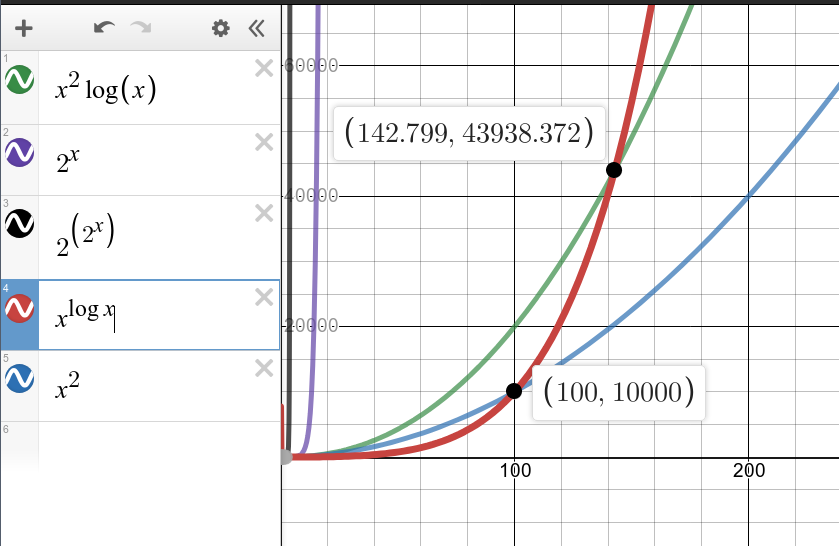
\includegraphics[scale=0.5]{p5/p5.png}
    \caption{Plot of all functions}
    \label{p5_plot}
\end{figure}

According to the graph the order will be: (Increasing order of grow rate)\\

\begin{enumerate}
    \item $n^{2}$ (Lesser order of grow rate)
    \item $n^{2}log(n)$
    \item $n^{log(n)}$
    \item $2^{n}$
    \item $2^{2^{n}}$ (Higher order of grow rate)
\end{enumerate}

\emph{Commentaries: }

As we can see in the plot the function $2^{2^{n}}$ grow fastest passing 60000 with only $x \approx 8$ that mean it is $\mathcal{O}()$ of the rest of functions. After $2^{2^{n}}$ comes $2^{n}$ with high grow rate passing 60000 with only $x \approx 18$. The rest of functions require more analyses because on the beginning of the domain looks like $n^{2}log(n)$ have more grow rate than the rest; however, as the value of $x$ grow the situation changes. Since we use an $x$ big enough to obtain the order of grow, we need to zoom out the plot. With a $x$ big enough we can see the function $n^{log(n)}$ pass $n^{2}$ at $x = 100$ and pass $n^{2}log(n)$ at $x = 142.799$. That explain the order aforementioned.

\end{document}
